% Provenance (never printed): old terminale S material on the early Earth (the
% primitive atmosphere and its outgassing, the first traces of life, the rise of
% oxygen read in the rocks: banded iron formations, red beds) and the faint young
% Sun. Owner (Sync 0/1): outgassing and primitive atmosphere, faint young Sun
% problem, stromatolite, Great Oxidation Event, banded iron formation, red beds.
% Recalled: age of the Earth (g12.07), zircons (g12.01), equilibrium temperature
% (g10.02), photosynthesis and cyanobacteria (biology), air composition, greenhouse
% gases as molecules and redox (chemistry). Figures: figdata/grade-12/early_earth.py.
\chapter{आरंभिक पृथ्वी और उसका वायुमंडल}\label{ch:g12:early-earth}

उत्तर-पश्चिमी ऑस्ट्रेलिया की हैमर्सली पर्वतमाला में डेल्स गॉर्ज की दीवारें
परतदार केक की तरह धारीदार हैं: लाल, धूसर और काली चट्टान की पतली पट्टियाँ। वे
एक \omterm{def:g12:early-earth:bif}{पट्टित लौह संरचना} हैं, जो 2.5 अरब वर्ष से भी पहले किसी समुद्र-तल पर
निक्षेपित हुई।
उनका लोहा उस समुद्र में जंग खा गया, और जंग लगने के लिए उसे ऑक्सीजन चाहिए थी। यह
अध्याय पूछता है कि युवा पृथ्वी और उसकी वायु कैसी थीं, और चट्टानें
उस क्षण को कैसे दर्ज करती हैं जब ऑक्सीजन प्रकट हुई।
% ledger: dbca:karijini, earle:bif, photo:g12-dales-gorge

\begin{omfigure}
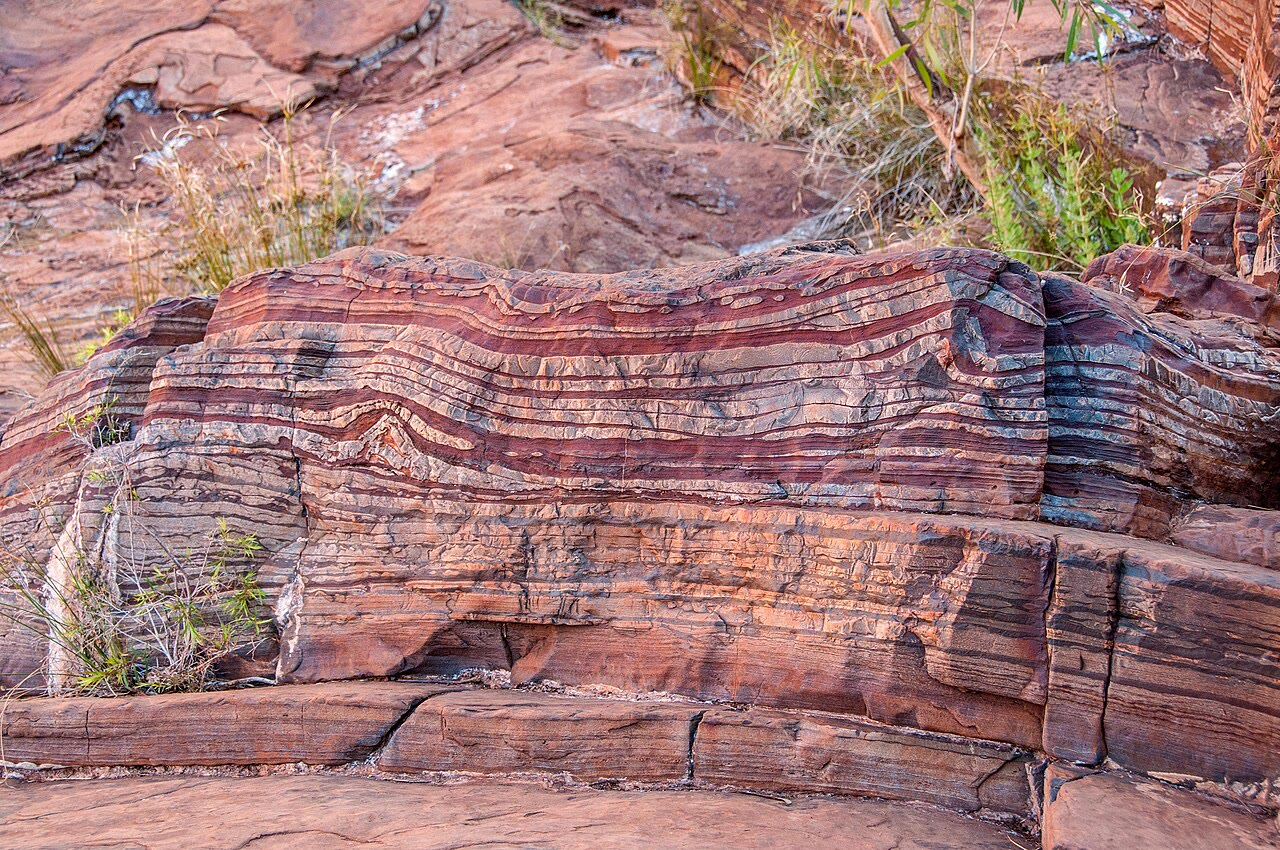
\includegraphics[width=0.72\linewidth]{images/book2/g12-dales-gorge-bif.jpg}

{\small फ़ोर्टेस्क्यू फ़ॉल्स, डेल्स गॉर्ज, करिजिनी राष्ट्रीय उद्यान, पश्चिमी
ऑस्ट्रेलिया में \omterm{def:g12:early-earth:bif}{पट्टित लौह संरचना}। फ़ोटो ग्रेम चर्चर्ड, CC~BY~2.0
(विकिमीडिया कॉमन्स)।}
\end{omfigure}

\begin{recall}
पृथ्वी 4.54 अरब वर्ष पुरानी है (\cref{ch:g12:age-of-the-earth}), और
ज़र्कॉन दिखाते हैं कि 4.4 अरब वर्ष पहले एक भूपर्पटी मौजूद थी
(\cref{ch:g12:continental-crust})। किसी ग्रह का \omterm{def:g10:habitable-planet:equilibrium-temperature}{साम्य तापमान},
$T_{\mathrm{eq}} = \left(S(1-A)/(4\sigma)\right)^{1/4}$, आज की पृथ्वी के लिए लगभग \qty{255}{K}
है (\cref{ch:g10:habitable-planet})। आज की शुष्क वायु में
\qty{78}{\percent} नाइट्रोजन और \qty{21}{\percent} ऑक्सीजन है, और कार्बन डाइऑक्साइड और
मीथेन ग्रीनहाउस गैसें हैं; जो तत्त्व ऑक्सीजन ग्रहण करता है, वह ऑक्सीकृत होता है (रसायन
की पुस्तकें)। पौधे, शैवाल और सायनोबैक्टीरिया अपना भोजन
प्रकाशसंश्लेषण द्वारा बनाते हैं, जो ऑक्सीजन मुक्त करता है (जीव विज्ञान की पुस्तकें)।
\end{recall}
% ledger: usgs:age-earth (Book 1 row), wilde01:zircon, earth:TSI, earth:albedo, air:N2, air:O2

\section{युवा पृथ्वी}

पृथ्वी छोटे पिंडों की अभिवृद्धि से बढ़ी। सौर मंडल के बनना शुरू होने के लगभग 60 मिलियन वर्ष
बाद, शायद मंगल के आकार का एक पिंड उससे टकराया,
और अंतरिक्ष में उछाले गए पदार्थ से चंद्रमा बना। युवा पृथ्वी
गरम थी और अभी आंशिक रूप से पिघली हुई थी। वह ठंडी हुई, और लगभग 4.4 अरब वर्ष पहले तक उसके
पास भूपर्पटी और महासागर दोनों थे: उस आयु के ज़र्कॉन तरल जल का रासायनिक
चिह्न लिए हुए हैं।
% ledger: nasa:moon-formation, wilde01:zircon

\section{आदिम वायुमंडल}

\begin{definition}[बहिर्गैसन; आदिम वायुमंडल]\label{def:g12:early-earth:primitive-atmosphere}
\emph{बहिर्गैसन}\index{बहिर्गैसन} ज्वालामुखियों द्वारा और भूमि के रास्ते
मैग्मा में घुली गैसों का मुक्त होना है। \emph{आदिम
वायुमंडल}\index{आदिम वायुमंडल} जीवों द्वारा बदले जाने से पहले का पृथ्वी का
वायुमंडल है: मुख्यतः बहिर्गैसन से बना, उसमें नाइट्रोजन,
कार्बन डाइऑक्साइड और जलवाष्प थे, आज से अधिक कार्बन डाइऑक्साइड, और लगभग
कोई मुक्त ऑक्सीजन नहीं।
\end{definition}
% ledger: usgs:volcanic-gases (Book 1 row), holland06:stages (stage 1 anoxic), feulner12:fys (more carbon dioxide)

ज्वालामुखी आज भी दिखाते हैं कि ऐसा वायुमंडल कैसे बनता है: जैसे-जैसे मैग्मा ऊपर उठता है और
दाब घटता है, उसकी घुली गैसें निकल जाती हैं, जिनमें कहीं सबसे प्रचुर
जलवाष्प है, फिर कार्बन डाइऑक्साइड। नाइट्रोजन और कार्बन डाइऑक्साइड, वे गैसें
जो आदिम वायु पर हावी थीं, आज भी ज्वालामुखियों की मुख्य नाइट्रोजन- और
कार्बन-युक्त गैसें हैं। जलवाष्प संघनित होकर
महासागर बनी। ऑक्सीजन आज की वायु में उसके स्तर के \qty{0.001}{\percent} से भी कम
थी।
% ledger: usgs:volcanic-gases (Book 1 row), pk02:anoxic

युवा सूर्य आज से कम चमकता था। जैसे-जैसे वह अपने क्रोड में हाइड्रोजन को
हीलियम में बदलता है, क्रोड सिकुड़ता और गरम होता है, और सूर्य की शक्ति
धीरे-धीरे बढ़ती है।

\begin{proposition}[युवा सूर्य की दीप्ति]\label{prop:g12:early-earth:luminosity}
$t_\odot$ को सूर्य की वर्तमान आयु और $L_\odot$ को उसकी वर्तमान
दीप्ति कहें, तो जब वह $t$ वर्ष का था, तब उसकी दीप्ति थी
\[
  L(t) = \frac{L_\odot}{1 + \frac{2}{5}\left(1 - t/t_\odot\right)} .
\]
\end{proposition}
% ledger: gough81:luminosity, connelly12:cai

सूर्य के अभिकलित मॉडलों का यह सन्निकटन यहाँ मान लिया गया है।
सूर्य के जन्म पर, $t = 0$, यह $L = L_\odot/1.4 \approx 0.71\,L_\odot$ देता है:
युवा सूर्य लगभग \qty{30}{\percent} मंद था।

\begin{example}[चार अरब वर्ष पहले की पृथ्वी]\label{ex:g12:early-earth:young-sun}
$t_\odot = 4.567$ अरब वर्ष लीजिए। चार अरब वर्ष पहले सूर्य
0.567 अरब वर्ष का था, इसलिए $1 - t/t_\odot = 4/4.567 \approx 0.876$ और
$L \approx L_\odot/1.350 \approx 0.741\,L_\odot$। पृथ्वी तक पहुँचने वाला
सूर्य-प्रकाश $0.741 \times 1361 \approx \qty{1008}{W/m^2}$ था। आज का
\omterm{def:g10:earth-energy-budget:albedo}{एल्बिडो} रखने पर, \omterm{def:g10:habitable-planet:equilibrium-temperature}{साम्य तापमान} सूर्य-प्रकाश के चतुर्थ मूल के अनुपात में
बदलता है: $255 \times 0.741^{1/4} \approx 255 \times 0.928 \approx
\qty{237}{K}$, लगभग \qty{-36}{\celsius}।
\end{example}
% values: L_4Ga 0.7406, S_4Ga 1007.9, Teq_today 255.1, Teq_4Ga 236.7 (early_earth.py)

\begin{omfigure}
\begin{tikzpicture}
\begin{axis}[omrecord, scale only axis, width=0.66\linewidth, height=4.6cm,
  xmin=0, xmax=4.6, ymin=225, ymax=295, x dir=reverse, axis y line*=left,
  xlabel={वर्तमान से पहले का समय (अरब वर्ष)}, ylabel={तापमान (K)},
  xtick={0,0.5,...,4.5}, x tick label style={/pgf/number format/.cd, fixed, precision=1}]
% computed in figdata/grade-12/early_earth.py; ledger: gough81:luminosity, earth:TSI, earth:albedo, earth:Tsurf
\addplot[omDef, line width=1.2pt] table[x=t_Ga, y=Teq] {figdata/out/grade-12-early_earth-sun.dat};
\addplot[omThm, densely dashed, domain=0:4.6, samples=2] {273.15};
\addplot[black!60, densely dotted, domain=0:4.6, samples=2] {288};
\coordinate (teq) at (axis cs:2.6,239);
\coordinate (frz) at (axis cs:2.3,274);
\coordinate (sfc) at (axis cs:2.3,289);
\end{axis}
\begin{axis}[omrecord, scale only axis, width=0.66\linewidth, height=4.6cm,
  xmin=0, xmax=4.6, ymin=0.65, ymax=1.05, x dir=reverse, axis y line*=right, axis x line=none,
  ylabel={सूर्य की दीप्ति ($L_\odot$)}, ymajorgrids=false, xmajorgrids=false,
  y tick label style={/pgf/number format/.cd, fixed, fixed zerofill, precision=2}]
\addplot[omProp, line width=0.9pt, densely dashdotted] table[x=t_Ga, y=L] {figdata/out/grade-12-early_earth-sun.dat};
\coordinate (lum) at (axis cs:1.7,0.86);
\end{axis}
\node[font=\scriptsize, text=omDef, anchor=north] at (teq) {साम्य तापमान};
\node[font=\scriptsize, text=omThm, anchor=south] at (frz) {जल जमता है, \qty{273}{K}};
\node[font=\scriptsize, text=black!70, anchor=south] at (sfc) {आज का माध्य सतह-तापमान, \qty{288}{K}};
\node[font=\scriptsize, text=omProp, anchor=north west] at (lum) {दीप्ति (दायाँ पैमाना)};
\end{tikzpicture}

{\small मंद युवा सूर्य: उसकी दीप्ति (दायाँ पैमाना) और आज के \omterm{def:g10:earth-energy-budget:albedo}{एल्बिडो} के साथ पृथ्वी का
\omterm{def:g10:habitable-planet:equilibrium-temperature}{साम्य तापमान} (बायाँ पैमाना), सूर्य के जन्म तक पीछे।
गफ़ (1981) से, आज के सूर्य-प्रकाश और \omterm{def:g10:earth-energy-budget:albedo}{एल्बिडो} के साथ परिकलित।}
\end{omfigure}

\begin{definition}[मंद युवा सूर्य की समस्या]\label{def:g12:early-earth:faint-young-sun}
\emph{मंद युवा सूर्य की समस्या}\index{मंद युवा सूर्य की समस्या} पृथ्वी के पहले कुछ अरब वर्षों के
मंद सूर्य, जिसके नीचे आज के वायुमंडल वाली पृथ्वी जम गई होती, और
उन चट्टानों के बीच का विरोधाभास है जो दिखाती हैं कि तरल जल मौजूद था।
\end{definition}
% ledger: feulner12:fys

इस समस्या को 1972 में कार्ल सेगन और जॉर्ज म्यूलेन ने व्यापक रूप से ज्ञात कराया,
जिन्होंने उत्तर के रूप में अधिक प्रबल ग्रीनहाउस प्रभाव प्रस्तावित किया। तब से अध्ययन किए गए अधिकांश
उत्तर \omterm{def:g12:early-earth:primitive-atmosphere}{आदिम वायुमंडल} में अधिक ग्रीनहाउस गैसों का सहारा लेते हैं:
आज से कहीं अधिक कार्बन डाइऑक्साइड, आरंभिक सूक्ष्मजीवों द्वारा बनी मीथेन, या
दोनों। एक प्रसिद्ध परिकलन में, कार्बन डाइऑक्साइड का लगभग दसवाँ भाग बार,
थोड़ी मीथेन के साथ, युवा पृथ्वी को आज जितना गरम रखता है; मीथेन के
बिना, लगभग तीन गुना अधिक चाहिए। इस समस्या को अभी
हल हुआ नहीं माना जाता।
% ledger: feulner12:fys

\section{जीवन और ऑक्सीजन}

\omterm{def:g12:early-earth:stromatolite}{स्ट्रोमैटोलाइटों} का जीवाश्म अभिलेख लगभग \num{3500} मिलियन वर्षों में फैला है:
वे जीवन के सबसे पुराने चिह्नों में से हैं।

\begin{definition}[स्ट्रोमैटोलाइट]\label{def:g12:early-earth:stromatolite}
\emph{स्ट्रोमैटोलाइट}\index{स्ट्रोमैटोलाइट} उथले जल में सूक्ष्मजीवों की, मुख्यतः
सायनोबैक्टीरिया की, एक चटाई द्वारा बनाया गया परतदार टीला है, जो अवसाद के कणों को फँसाकर
बाँधती है और कार्बोनेट को परत-दर-परत बढ़ाती है।
\end{definition}
% ledger: noffke13:stromatolites

\num{3430} मिलियन वर्ष पुराने जीवाश्म \omterm{def:g12:early-earth:stromatolite}{स्ट्रोमैटोलाइट} पश्चिमी ऑस्ट्रेलिया के पिलबारा के
स्ट्रेली पूल चर्ट में मिलते हैं। जीवित \omterm{def:g12:early-earth:stromatolite}{स्ट्रोमैटोलाइट} आज शार्क बे के
हैमेलिन पूल के बहुत खारे जल में बढ़ते हैं, जो सामान्य समुद्री जल से दुगुना खारा है,
जहाँ वे सबसे प्रसिद्ध आधुनिक उदाहरण हैं।
% ledger: allwood06:spc, noffke13:stromatolites, dbca:hamelin

\begin{omfigure}
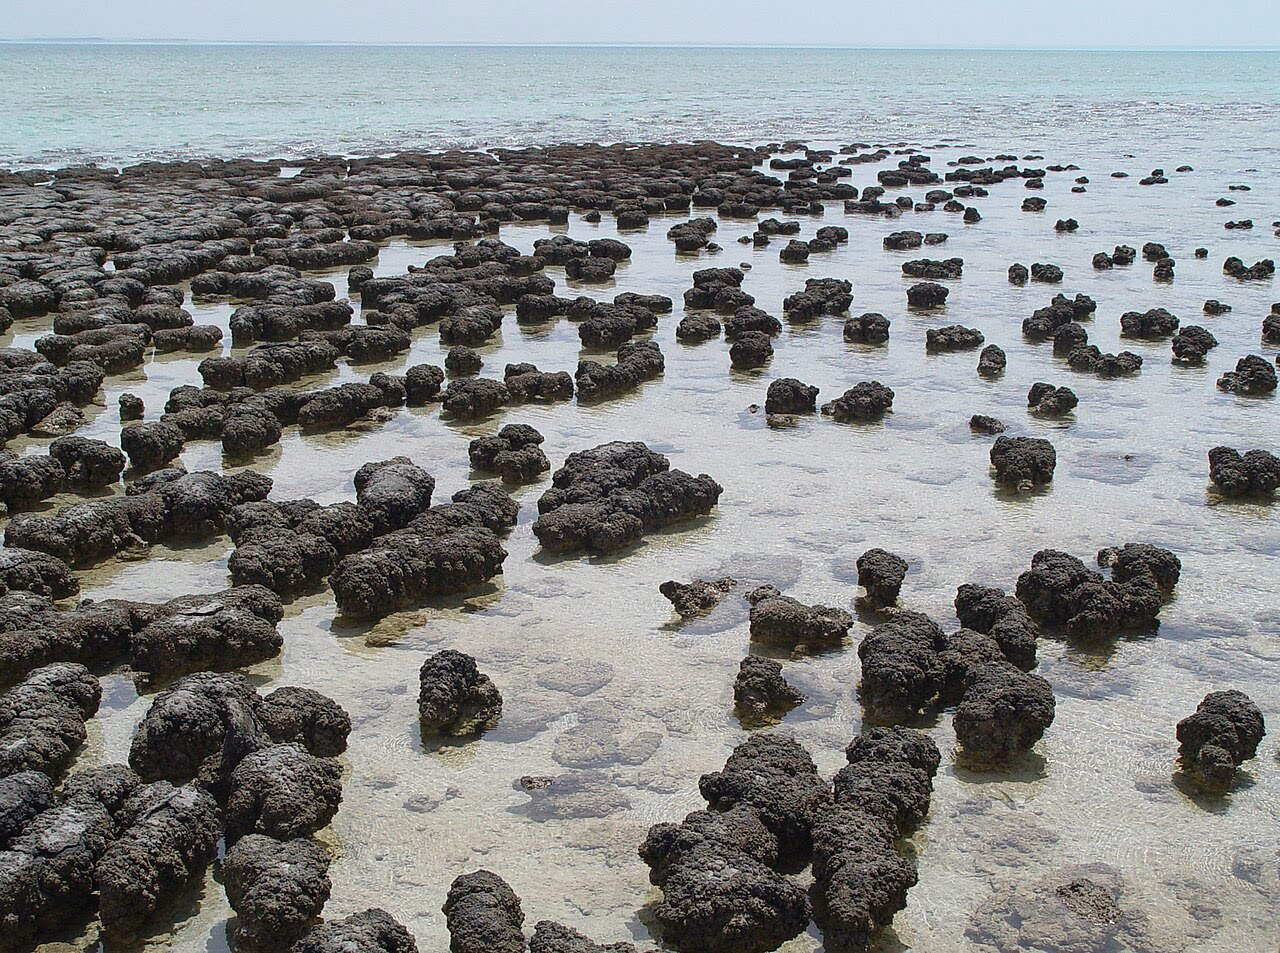
\includegraphics[width=0.6\linewidth]{images/book2/g12-shark-bay-stromatolites.jpg}

{\small हैमेलिन पूल, शार्क बे, पश्चिमी ऑस्ट्रेलिया में जीवित \omterm{def:g12:early-earth:stromatolite}{स्ट्रोमैटोलाइट}।
फ़ोटो पॉल हैरिसन, CC~BY-SA~3.0 (विकिमीडिया कॉमन्स)।}
\end{omfigure}
% ledger: photo:g12-shark-bay

सायनोबैक्टीरिया कुछ नया लाए: ऐसा प्रकाशसंश्लेषण जो ऑक्सीजन
मुक्त करता है। पर लंबे समय तक उनकी बनाई ऑक्सीजन वायु में नहीं टिकी। वह
उतनी ही तेज़ी से खप जाती थी जितनी तेज़ी से बनती थी: समुद्र में घुले लोहे द्वारा,
गंधक द्वारा और मीथेन द्वारा।

\section{ऑक्सीजन का उदय}

ऑक्सीजन से पहले, लोहा समुद्री जल में घुलकर आयन
\ce{Fe^2+} के रूप में यात्रा कर सकता था। ऑक्सीजन उसे आयरन(III) में बदल देती है, जो घुलता नहीं: वह
जंग-जैसे अवसाद के रूप में तल पर गिर जाता है।

\begin{proposition}[लोहा ऑक्सीजन ग्रहण करता है]\label{prop:g12:early-earth:iron}
घुला हुआ आयरन(II) जल में ऑक्सीजन द्वारा ऑक्सीकृत होकर आयरन(III) हाइड्रॉक्साइड बनता है,
जो अवक्षेपित होता है:
\[
  \ce{4Fe^2+ + O2 + 10H2O -> 4Fe(OH)3 + 8H+} .
\]
ऑक्सीजन का हर अणु घुले लोहे के चार आयन हटाता है; जब तक
घुला लोहा बचा रहता है, बनी हुई ऑक्सीजन खप जाती है।
\end{proposition}
% ledger: earle:bif (ferrous iron oxidised to insoluble ferric iron)

\begin{proof}
संतुलन जाँचिए। लोहा: हर ओर 4। ऑक्सीजन: बाईं ओर $2 + 10 = 12$,
दाईं ओर $4 \times 3 = 12$। हाइड्रोजन: बाईं ओर $20$, दाईं ओर $4 \times 3 + 8 =
20$। आवेश: बाईं ओर $4 \times (+2) = +8$, दाईं ओर $8 \times (+1) =
+8$।
\end{proof}

\begin{definition}[पट्टित लौह संरचना]\label{def:g12:early-earth:bif}
\emph{पट्टित लौह संरचना}\index{पट्टित लौह संरचना} एक
अवसादी चट्टान है जिसमें लौह ऑक्साइडों, जैसे
हेमेटाइट, और चर्ट, लोहे में निर्धन एक महीन-कणीय सिलिका, की पतली एकांतर परतें होती हैं। लगभग सभी
1.8 अरब वर्ष से पुरानी हैं।
\end{definition}
% ledger: earle:bif, holland06:stages

\omterm{def:g12:early-earth:bif}{पट्टित लौह संरचनाओं} को एक साथ दो जलों की आवश्यकता होती है: ऑक्सीजन-रहित एक \omterm{def:g10:layered-ocean:thermocline}{गहन महासागर},
जो घुला लोहा ले जाता है, और एक उथला, धूप वाला समुद्र जहाँ सायनोबैक्टीरिया
ऑक्सीजन बनाते हैं और लोहा अवक्षेपित होता है। वे 2.4 से
1.8 अरब वर्ष पुरानी चट्टानों में आम हैं, और हैमर्सली पर्वतमाला की संरचनाएँ उनसे भी पुरानी हैं।
\omterm{def:g12:early-earth:bif}{पट्टित लौह संरचनाएँ} लोहे का एक आम अयस्क हैं।
% ledger: earle:bif, holland06:stages (Archean BIF, Hamersley), dbca:karijini

\begin{omfigure}
\begin{tikzpicture}[x=1cm, y=1cm, font=\scriptsize]
  % sea and floor
  \fill[omSea] (0,0) rectangle (11,4);
  \fill[omSea!45!white] (0,2.9) rectangle (11,4);
  \draw[omDef!60, line width=0.4pt, densely dashed] (0,2.9) -- (11,2.9);
  \node[anchor=north east, text=omDef] at (10.9,3.95) {धूप वाला सतही जल};
  \node[anchor=south east, text=omDef, align=right] at (10.9,0.12) {ऑक्सीजन-रहित\\गहरा जल,\\\ce{Fe^2+} से समृद्ध};
  % floor with layers
  \foreach \i/\c in {0/red!55!black, 1/black!20, 2/red!55!black, 3/black!20, 4/red!55!black, 5/black!20} {
    \fill[\c] (0,-0.12*\i) rectangle (11,-0.12*\i-0.12);
  }
  \draw[black!60] (0,0) -- (11,0);
  \node[anchor=west] at (11.1,-0.12) {लौह ऑक्साइड};
  \node[anchor=west] at (11.1,-0.36) {चर्ट};
  \draw[black!50, line width=0.3pt] (11.05,-0.06) -- (10.6,-0.06);
  \draw[black!50, line width=0.3pt] (11.05,-0.30) -- (10.6,-0.30);
  % upwelling iron
  \foreach \x in {0.5,1.0,1.5} {
    \draw[-{Stealth}, omDef, line width=0.8pt] (\x,0.4) .. controls (\x+0.4,1.5) and (\x+0.6,2.2) .. (\x+0.9,2.85);
  }
  \node[text=omDef, anchor=west] at (2.3,1.3) {\ce{Fe^2+} ऊपर उठता है};
  % cyanobacteria and oxygen
  \foreach \x in {3.8,4.4,5.0,5.6,6.2} {\fill[green!45!black] (\x,3.35) circle (0.07);}
  \node[anchor=south, text=green!35!black] at (5.0,3.47) {सायनोबैक्टीरिया \ce{O2} बनाते हैं};
  % reaction
  \node[draw=black!40, fill=white, rounded corners=2pt, inner sep=2pt] at (5.4,2.45) {\ce{4Fe^2+ + O2 + 10H2O -> 4Fe(OH)3 + 8H+}};
  % falling rust
  \foreach \x/\y in {4.6/1.9, 5.0/1.5, 5.5/1.8, 5.9/1.2, 4.3/1.1, 5.2/0.7, 6.1/0.6} {\fill[red!60!black] (\x,\y) circle (0.06);}
  \draw[-{Stealth}, red!60!black, line width=0.6pt] (6.6,2.1) -- (6.6,0.25);
  \node[anchor=west, text=red!60!black, align=left] at (6.7,1.75) {आयरन(III) जंग-जैसी\\परत बनकर बैठता है};
\end{tikzpicture}

{\small \omterm{def:g12:early-earth:bif}{पट्टित लौह संरचना} कैसे बनती है (योजनाबद्ध, पैमाने पर नहीं): गहरे जल में,
जिसमें कोई ऑक्सीजन नहीं, घुला लोहा धूप वाले समुद्र में ऊपर उठता है,
जहाँ सायनोबैक्टीरिया द्वारा बनी ऑक्सीजन उसे आयरन(III) में बदल देती है, जो
नीचे बैठ जाता है। लोहे से समृद्ध परतें चर्ट की परतों के साथ बारी-बारी से आती हैं।}
\end{omfigure}

फिर ऑक्सीजन वायु में टिकने लगी।

\begin{definition}[महा ऑक्सीकरण घटना]\label{def:g12:early-earth:goe}
\emph{महा ऑक्सीकरण घटना}\index{महा ऑक्सीकरण घटना} वह
अंतराल है, लगभग \num{2.46} से लगभग \num{2.06} अरब वर्ष पहले तक, जिसके दौरान
मुक्त ऑक्सीजन पहली बार पृथ्वी के वायुमंडल और उथले समुद्रों में संचित हुई,
और शायद अपने वर्तमान स्तर के दसवें भाग तक पहुँची।
\end{definition}
% ledger: gumsley17:goe, holland06:stages (0.02-0.04 atm, about a tenth of 0.21)

प्रमाण चट्टानों में है। कुछ खनिज, जिनमें पाइराइट और यूरेनिनाइट
भी हैं, ऑक्सीजन से नष्ट हो जाते हैं; फिर भी नदियों द्वारा लुढ़काए गए उनके कण
पुराने अवसादों में मिलते हैं, और पाइराइट के कण ऑक्सीजन के उदय के बाद निक्षेपित
अवसादों से ग़ायब हैं। लगभग 2.45 अरब वर्ष से पुरानी चट्टानों में गंधक के समस्थानिक एक
ऐसा चिह्न लिए हुए हैं जो केवल वह वायु छोड़ सकती है जिसमें आज की
ऑक्सीजन के एक लाखवें भाग से कम हो; 2.09 अरब वर्ष पहले तक वह ग़ायब हो चुका है। और भूमि पर
\omterm{def:g12:early-earth:red-beds}{लाल संस्तर} प्रकट हुए।
% ledger: kasting25:indicators, pk02:anoxic, farquhar00:sulfur

\begin{definition}[लाल संस्तर]\label{def:g12:early-earth:red-beds}
\emph{लाल संस्तर}\index{लाल संस्तर} वे अवसादी चट्टानें हैं --- बलुआ पत्थर,
गादाश्म, शेल --- जो अपने कणों पर आयरन(III) ऑक्साइड, हेमेटाइट, की परत से
लाल रंगी होती हैं। वे केवल वहीं बनते हैं जहाँ लोहे को ऑक्सीकृत करने के लिए
पर्याप्त ऑक्सीजन हो।
\end{definition}
% ledger: kasting25:indicators (redbeds an oxygen indicator)

\begin{omfigure}
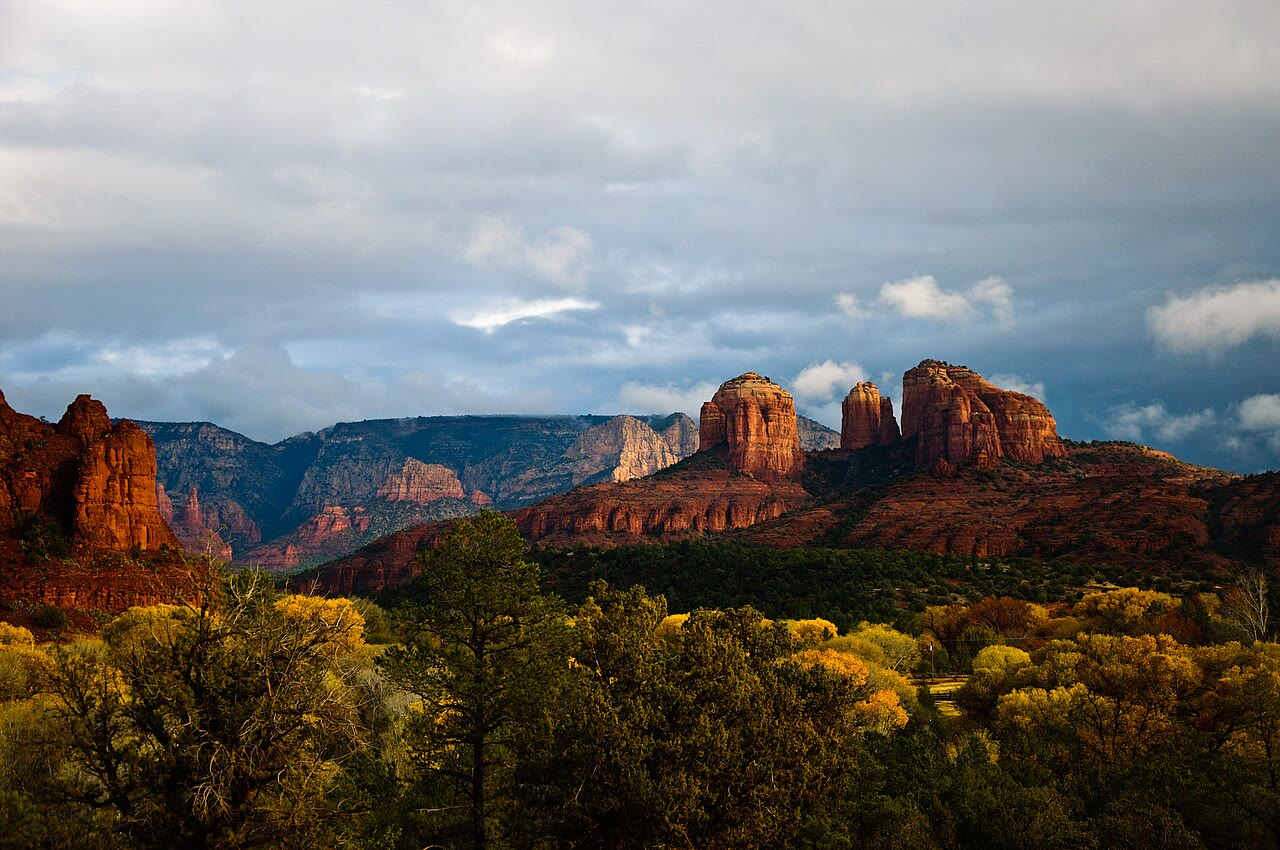
\includegraphics[width=0.66\linewidth]{images/book2/g12-sedona-red-beds.jpg}

{\small \omterm{def:g12:early-earth:red-beds}{लाल संस्तर}: सेडोना, एरिज़ोना के निकट कैथेड्रल रॉक, जो पर्मियन लाल
बलुआ पत्थरों से बना है। फ़ोटो वेंडी फ़्रॉम पेनसिल्वेनिया, CC~BY-SA~2.0 (विकिमीडिया
कॉमन्स)।}
\end{omfigure}
% ledger: photo:g12-sedona, azgs:cathedral (Permian Schnebly Hill Sandstone)

1.8 अरब वर्ष पहले के बाद \omterm{def:g12:early-earth:bif}{पट्टित लौह संरचनाओं} का बनना लगभग रुक गया:
तब तक \omterm{def:g10:layered-ocean:thermocline}{गहन महासागर} में भी इतनी ऑक्सीजन थी कि वह
लोहा ले जाना बंद कर दे। अगले एक अरब वर्ष में ऑक्सीजन थोड़ी ही बदली; 0.85 अरब
वर्ष पहले के बाद वह फिर बढ़ी, आज के \qty{21}{\percent} की ओर।
% ledger: earle:bif, holland06:stages

\begin{method}[भूवैज्ञानिक समयरेखा पढ़ना]\label{met:g12:early-earth:timeline}
\begin{enumerate}
  \item पता कीजिए कि अक्ष पर समय किस ओर चलता है, और उसकी इकाई क्या है (वर्तमान से
        पहले के मिलियन या अरब वर्ष)।
  \item रंगीन पट्टी पर इयॉन ढूँढ़िए, और उनकी सीमाएँ पढ़िए।
  \item हर घटना की तिथि पढ़िए, या वह अंतराल जिसके दौरान वह
        हुई, और बताइए कि कौन-सा अभिलेख उसकी तिथि देता है (कोई खनिज, कोई जीवाश्म, कोई चट्टान)।
  \item घटाकर अवधियाँ परिकलित कीजिए, और उनकी तुलना \omterm{def:g12:age-of-the-earth:age}{पृथ्वी की
        आयु} से कीजिए।
  \item क्रम जाँचिए: कोई प्रभाव अपने कारण से पहले नहीं आना चाहिए।
\end{enumerate}
\end{method}

\begin{omfigure}
\begin{tikzpicture}
\begin{axis}[omrecord, width=0.82\linewidth, height=6.2cm, ymode=log, xmin=0, xmax=4.6, ymin=1e-7, ymax=5,
  x dir=reverse, xlabel={वर्तमान से पहले का समय (अरब वर्ष)}, ylabel={वायु में ऑक्सीजन (आज $=1$)},
  xtick={0,0.5,...,4.5}, x tick label style={/pgf/number format/.cd, fixed, precision=1},
  ytick={1e-6,1e-4,1e-2,1}, ymajorgrids=true, xmajorgrids=false, clip=false]
% computed in figdata/grade-12/early_earth.py (schematic through the sourced bounds); ledger: holland06:stages, pk02:anoxic, gumsley17:goe, ics:base.Hadean, ics:base.Archean, ics:base.Proterozoic, ics:base.Paleozoic
\fill[omThm!12] (axis cs:2.46,1e-7) rectangle (axis cs:2.06,5);
\addplot[black, line width=1.2pt] table[x=t_Ga, y=pal] {figdata/out/grade-12-early_earth-oxygen.dat};
% eon band (ICS colours), below the axis
\fill[icsHadean] (axis cs:4.567,1.5e-7) rectangle (axis cs:4.031,4e-7);
\fill[icsArchean] (axis cs:4.031,1.5e-7) rectangle (axis cs:2.5,4e-7);
\fill[icsProterozoic] (axis cs:2.5,1.5e-7) rectangle (axis cs:0.5388,4e-7);
\fill[icsPhanerozoic] (axis cs:0.5388,1.5e-7) rectangle (axis cs:0,4e-7);
\node[font=\tiny, text=white] at (axis cs:4.30,2.45e-7) {हेडियन};
\node[font=\tiny, text=white] at (axis cs:3.27,2.45e-7) {आर्कियन};
\node[font=\tiny, text=white] at (axis cs:1.52,2.45e-7) {प्रोटेरोज़ोइक};
% events
\draw[omDef, line width=0.6pt] (axis cs:4.4,4e-7) -- (axis cs:4.4,3e-3);
\node[font=\scriptsize, text=omDef, anchor=south west] at (axis cs:4.4,3e-3) {ज़र्कॉन, जल};
\draw[omMeth, line width=0.6pt] (axis cs:3.43,4e-7) -- (axis cs:3.43,1.2e-6);
\node[font=\scriptsize, text=omMeth, anchor=south] at (axis cs:3.43,1.2e-6) {पहले स्ट्रोमैटोलाइट};
\draw[red!60!black, line width=3pt] (axis cs:2.4,3e-6) -- (axis cs:1.8,3e-6);
\node[font=\scriptsize, text=red!60!black, anchor=north] at (axis cs:2.16,2.4e-6) {पट्टित लौह संरचनाएँ};
\node[font=\scriptsize, text=omThm, anchor=south, align=center] at (axis cs:2.26,1.2) {महा ऑक्सीकरण\\घटना};
\node[font=\scriptsize, anchor=south] at (axis cs:3.2,1.3e-5) {आज के $10^{-5}$ से कम};
\node[font=\scriptsize, anchor=south] at (axis cs:1.4,0.12) {लगभग दसवाँ भाग};
\end{axis}
\end{tikzpicture}

{\small समय के साथ वायु में ऑक्सीजन (योजनाबद्ध, लघुगणकीय पैमाना):
वक्र मापी गई सीमाओं को जोड़ता है और वास्तविक अभिलेख के उतार-चढ़ाव छिपा देता है।
छायांकित अंतराल \omterm{def:g12:early-earth:goe}{महा ऑक्सीकरण घटना} है; लाल पट्टी
वह समय दिखाती है जब \omterm{def:g12:early-earth:bif}{पट्टित लौह संरचनाएँ} आम थीं, 2.4 से 1.8 अरब वर्ष
पहले। इयॉन अंतरराष्ट्रीय
कालस्तरिकी चार्ट से।}
\end{omfigure}

\section{अभ्यास}

\begin{exercise}[$\star$]\label{exo:g12:early-earth:1}
शब्द बताइए: (a) मैग्मा में घुली गैसों का मुक्त होना; (b) सूक्ष्मजीवी चटाई द्वारा बना
परतदार टीला; (c) लौह ऑक्साइड और चर्ट की एकांतर परतों वाली चट्टान;
(d) हेमेटाइट से रंगी अवसादी चट्टानें; (e) वह अंतराल
जब वायु में पहली बार ऑक्सीजन संचित हुई।
\end{exercise}

\begin{exercise}[$\star$]\label{exo:g12:early-earth:2}
सबसे पुरानी से शुरू करके क्रम में रखिए: अधिकांश \omterm{def:g12:early-earth:bif}{पट्टित लौह संरचनाओं} का अंत;
पिलबारा के पहले \omterm{def:g12:early-earth:stromatolite}{स्ट्रोमैटोलाइट}; तरल जल दिखाने वाले ज़र्कॉन;
हैमर्सली की \omterm{def:g12:early-earth:bif}{पट्टित लौह संरचनाएँ}; \omterm{def:g12:early-earth:goe}{महा ऑक्सीकरण घटना} का अंत।
\end{exercise}

\begin{exercise}[$\star$]\label{exo:g12:early-earth:3}
दीप्ति-नियम का उपयोग करके, सूर्य के जन्म पर उसकी दीप्ति, आज की दीप्ति के
भिन्न के रूप में, परिकलित कीजिए। वह कितने प्रतिशत मंद था?
\end{exercise}

\begin{exercise}[$\star$]\label{exo:g12:early-earth:4}
नदियों द्वारा लुढ़काए गए पाइराइट के कण पुराने अवसादों में मिलते हैं, पर
ऑक्सीजन के उदय के बाद निक्षेपित अवसादों में नहीं। इससे पुराने अवसादों के समय की
वायु के बारे में आपको क्या पता चलता है? क्यों?
\end{exercise}

\begin{exercise}[$\star$]\label{exo:g12:early-earth:5}
ज्वालामुखियों द्वारा मुक्त की जाने वाली दो सबसे प्रचुर गैसों के नाम बताइए, और बताइए कि युवा
पृथ्वी में हर एक का क्या हुआ।
\end{exercise}

\begin{exercise}[$\star\star$]\label{exo:g12:early-earth:6}
$t_\odot = 4.567$ अरब वर्ष लेकर, 3 अरब वर्ष पहले और 2.45 अरब वर्ष पहले
सूर्य की दीप्ति और पृथ्वी का \omterm{def:g10:habitable-planet:equilibrium-temperature}{साम्य तापमान} (आज
\qty{255}{K}, \omterm{def:g10:earth-energy-budget:albedo}{एल्बिडो} अपरिवर्तित) परिकलित कीजिए।
\end{exercise}

\begin{exercise}[$\star\star$]\label{exo:g12:early-earth:7}
\qty{1}{kg} घुले लोहे को आयरन(III) हाइड्रॉक्साइड के रूप में अवक्षेपित करने के लिए
कितनी ऑक्सीजन चाहिए? (मोलर द्रव्यमान: लोहा \qty{55.85}{g/mol}, ऑक्सीजन
\qty{16.00}{g/mol}।)
\end{exercise}

\begin{exercise}[$\star\star$]\label{exo:g12:early-earth:8}
समयरेखा का उपयोग करके, (1) \omterm{def:g12:early-earth:goe}{महा ऑक्सीकरण घटना} कितने समय चली? (2)
पृथ्वी के इतिहास के कितने भाग में वायु में लगभग कोई ऑक्सीजन नहीं
थी? (3) पहले \omterm{def:g12:early-earth:stromatolite}{स्ट्रोमैटोलाइटों} के कितने समय बाद ऑक्सीजन संचित होने लगी?
\end{exercise}

\begin{exercise}[$\star\star$]\label{exo:g12:early-earth:9}
एक \omterm{def:g12:early-earth:bif}{पट्टित लौह संरचना} और एक \omterm{def:g12:early-earth:red-beds}{लाल संस्तर}, दोनों में आयरन(III) ऑक्साइड है। हर एक
ऑक्सीजन के बारे में आपको क्या बताता है, और कहाँ की: गहरे समुद्र की, उथले
समुद्र की, वायु की?
\end{exercise}

\begin{exercise}[$\star\star$]\label{exo:g12:early-earth:10}
जीवित \omterm{def:g12:early-earth:stromatolite}{स्ट्रोमैटोलाइट} आज कहाँ देखे जा सकते हैं? वहाँ के जल में क्या विशेष
है, और \omterm{def:g12:early-earth:stromatolite}{स्ट्रोमैटोलाइट} परत-दर-परत कैसे बढ़ता है?
\end{exercise}

\begin{exercise}[$\star\star$]\label{exo:g12:early-earth:11}
आज की वायु का \qty{21}{\percent} ऑक्सीजन है। जब वह (1) आज के स्तर का
एक लाखवाँ भाग थी; (2) आज के स्तर का दसवाँ भाग थी, तब वह कितने प्रतिशत थी?
\end{exercise}

\begin{exercise}[$\star\star\star$]\label{exo:g12:early-earth:12}
चार अरब वर्ष पहले, युवा सूर्य के नीचे ($L = 0.741\,L_\odot$,
आज का \omterm{def:g10:earth-energy-budget:albedo}{एल्बिडो} 0.294) कौन-सा \omterm{def:g10:earth-energy-budget:albedo}{एल्बिडो} पृथ्वी को आज का \omterm{def:g10:habitable-planet:equilibrium-temperature}{साम्य तापमान},
\qty{255}{K}, देता? क्या महासागर, बादलों और कुछ बर्फ़ वाला ग्रह
इतना गहरा रहा होगा? दूसरा उपाय क्या है?
\end{exercise}

\begin{exercise}[$\star\star\star$]\label{exo:g12:early-earth:13}
आज ग्रीनहाउस प्रभाव पृथ्वी की सतह को 255 से
\qty{288}{K} तक गरम करता है। चार अरब वर्ष पहले \omterm{def:g10:habitable-planet:equilibrium-temperature}{साम्य तापमान} लगभग
\qty{237}{K} था। (1) तब \qty{273}{K} तक पहुँचने के लिए कितने केल्विन की ग्रीनहाउस तापवृद्धि
चाहिए थी? \qty{288}{K} तक पहुँचने के लिए? (2) आज की तापवृद्धि से तुलना कीजिए।
(3) एक प्रसिद्ध परिकलन को लगभग \qty{0.1}{bar} कार्बन डाइऑक्साइड चाहिए,
थोड़ी मीथेन के साथ; इसकी तुलना आज के पूरे
वायुमंडल के दाब, लगभग \qty{1}{bar}, से कीजिए।
\end{exercise}

\begin{exercise}[$\star\star\star$]\label{exo:g12:early-earth:14}
गंधक के समस्थानिकों का एक विशेष चिह्न केवल तभी बन सकता है, और अवसादों में
सुरक्षित रह सकता है, जब वायु में आज की ऑक्सीजन के $10^{-5}$ से कम हो। यह
2450 मिलियन वर्ष से पुरानी चट्टानों में मिलता है, और 2090 मिलियन वर्ष से नई
चट्टानों में नहीं। (1) 2450 मिलियन वर्ष पहले से पहले की ऑक्सीजन के बारे में आप क्या
निष्कर्ष निकालते हैं? 2090 मिलियन वर्ष के बाद? (2) क्या यह \omterm{def:g12:early-earth:goe}{महा ऑक्सीकरण घटना} की
तिथियों से संगत है?
\end{exercise}

\begin{exercise}[$\star\star\star$]\label{exo:g12:early-earth:15}
चंद्रमा बनाने वाली टक्कर सौर मंडल के बनना शुरू होने के लगभग 60 मिलियन वर्ष बाद
हुई, जिसकी तिथि पहले ठोस 4567 मिलियन वर्ष पहले बताते हैं।
(1) टक्कर लगभग कब हुई? (2) सबसे पुराने ज़र्कॉन \num{4404}
मिलियन वर्ष पुराने हैं। टक्कर के अधिक से अधिक कितने समय बाद पृथ्वी के पास पहले से
ठोस भूपर्पटी और तरल जल थे?
\end{exercise}
% ledger: nasa:moon-formation, connelly12:cai, wilde01:4404

\begin{problem}[{सप्ताहांत समस्या --- मंद युवा सूर्य}]
\label{pb:g12:early-earth:1}
% ledger: gough81:luminosity, connelly12:cai, earth:TSI, earth:albedo, earth:Tsurf, feulner12:fys, allwood06:spc, dbca:karijini, wilde01:zircon
% values (early_earth.py): L_4Ga 0.7406, S_4Ga 1007.9, Teq_today 255.1, Teq_4Ga 236.7, albedo_needed 0.047
सूर्य \num{4.567} अरब वर्ष पुराना है। जब वह $t$
वर्ष का था, तब उसकी दीप्ति $L(t) = L_\odot/\bigl(1 + \tfrac25 (1 - t/t_\odot)\bigr)$ थी। आज
पृथ्वी \qty{1361}{W/m^2} सूर्य-प्रकाश पाती है, उसका 0.294 भाग परावर्तित करती है,
और उसका \omterm{def:g10:habitable-planet:equilibrium-temperature}{साम्य तापमान} \qty{255}{K} है; उसका माध्य सतह-तापमान
\qty{288}{K} है।

\medskip
\noindent\textbf{भाग I --- चार अरब वर्ष पहले का सूर्य।}
\begin{enumerate}
  \item चार अरब वर्ष पहले सूर्य की आयु कितनी थी?
  \item उस समय $1 - t/t_\odot$ परिकलित कीजिए।
  \item उसकी दीप्ति आज की दीप्ति के भिन्न के रूप में परिकलित कीजिए।
  \item पृथ्वी को कितना सूर्य-प्रकाश मिलता था, \unit{W/m^2} में?
  \item सूर्य आज की तुलना में कितने प्रतिशत मंद था?
\end{enumerate}

\medskip
\noindent\textbf{भाग II --- साम्य तापमान।}
\begin{enumerate}[resume]
  \item \omterm{def:g10:habitable-planet:equilibrium-temperature}{साम्य तापमान} को सूर्य-प्रकाश $S$ के फलन के रूप में लिखिए।
  \item दिखाइए कि \omterm{def:g10:earth-energy-budget:albedo}{एल्बिडो} अपरिवर्तित रहने पर तापमान
        $S^{1/4}$ के अनुसार बदलता है।
  \item $0.741^{1/4}$ परिकलित कीजिए।
  \item चार अरब वर्ष पहले का \omterm{def:g10:habitable-planet:equilibrium-temperature}{साम्य तापमान} परिकलित कीजिए।
  \item उसे डिग्री सेल्सियस में बदलिए।
\end{enumerate}

\medskip
\noindent\textbf{भाग III --- तरल जल के प्रमाण।}
\begin{enumerate}[resume]
  \item 4.4 अरब वर्ष पुराने ज़र्कॉन क्या दिखाते हैं?
  \item पिलबारा के \num{3430} मिलियन वर्ष पुराने \omterm{def:g12:early-earth:stromatolite}{स्ट्रोमैटोलाइट}
        किस प्रकार के जल में बढ़े?
  \item हैमर्सली पर्वतमाला की कौन-सी चट्टानें, जो 2.5 अरब वर्ष से भी पहले समुद्र में
        निक्षेपित हुईं, तरल जल माँगती हैं?
  \item ग्रीनहाउस प्रभाव के बिना, क्या चार अरब वर्ष पहले महासागर
        जम गया होता? क्यों?
  \item इससे प्रकट होने वाला विरोधाभास बताइए, और उसका नाम दीजिए।
\end{enumerate}

\medskip
\noindent\textbf{भाग IV --- आवश्यक ग्रीनहाउस तापवृद्धि।}
\begin{enumerate}[resume]
  \item आज का ग्रीनहाउस प्रभाव कितने केल्विन जोड़ता है?
  \item चार अरब वर्ष पहले माध्य सतह-तापमान को \qty{273}{K} से ऊपर
        रखने के लिए कितने केल्विन चाहिए थे?
  \item कौन-सा \omterm{def:g10:earth-energy-budget:albedo}{एल्बिडो} बिना किसी अतिरिक्त ग्रीनहाउस प्रभाव के \qty{255}{K}
        देता? क्या यह संभव है?
  \item माना जाता है कि अतिरिक्त तापवृद्धि का अधिकांश भाग किस गैस ने दिया, और
        किस दूसरी गैस ने सहायता की होगी?
  \item सारांश दीजिए: चार अरब वर्ष पहले पृथ्वी का \omterm{def:g10:habitable-planet:equilibrium-temperature}{साम्य तापमान} क्या
        था?
\end{enumerate}
\end{problem}
